\documentclass[12pt, a4paper]{article}
\usepackage[utf8]{inputenc}
\usepackage[brazil, english]{babel}
\usepackage[T1]{fontenc}
\usepackage{amsmath}
\usepackage{setspace}
\usepackage{indentfirst}
\usepackage{libertine}
\usepackage[natbibapa]{apacite}
\bibliographystyle{apacite}
\usepackage[left=2.5cm,top=3cm,right=2.5cm,bottom=2.5cm]{geometry}
\usepackage{lineno}
\usepackage{xcolor}
\usepackage{hyperref}
\usepackage{graphicx}

\definecolor{darkblue}{RGB}{255,10,10}


\usepackage{enumitem}

\newenvironment{hypothesis}
 {\enumerate[label=\textbf{H\arabic*.}, ref=H\arabic*]}
 {\endenumerate}
\makeatletter
\newcommand\varitem[1]{\item[\textbf{H\arabic{enumi}\rlap{$#1$}.}]%
  \edef\@currentlabel{H\arabic{enumi}{$#1$}}}
\makeatother


\title{\textbf{How Many Justices Does it Take to Control the Court?} A New Formal Argument for Understanding Judicial Independence}
\author{Guilherme Jardim Duarte\thanks{guilherme.duarte@jota.info}}

\hypersetup{pdftitle={How Many Justices Does it Take to Control the Court? A New Formal Argument for Understanding Judicial Independence},
	pdfauthor={Guilherme Jardim Duarte},
	pdfborder={0 0 0},
	breaklinks=true,
	linkcolor=darkblue,
	citecolor=darkblue,
	urlcolor=darkblue,
	colorlinks=true}

\date{\vspace{.5cm} \today \\ 
\vspace{.5cm} \textit{Preliminary draft --- please do not cite or circulate}}

\begin{document}
\doublespacing
\maketitle

\begin{abstract}


The literature on Judicial Politics has usually suggested that Presidents could guarantee their power over Supreme Courts provided that they nominated at least half of the bench. This theory relies on specific assumptions which
constitute the foundation of most Political Science studies on collective behavior. We argue, however, that those assumptions cannot always be replicated since individual justices have primacy over the collective body. The Brazilian Supreme Court is a good example, since there are a couple of institutional rules that allow
each justice to stop or change the result of a judgment without hearing his/her peers. In this setting, where individual behavior is underscored, there is a need for
a new theory to investigate how actors, including the President, can
influence the final result of a judgment. We develop in the current study a formal argument that subsumes those particularities. Finally, we derive implications for judicial independence studies. 


\vspace{.5cm}
\noindent
\textsc{Keywords}: Judicial Politics, Brazilian Supreme Court, Judicial Independence
\end{abstract}

\newpage

%\linenumbers
\section{Introduction}
  

Many studies in Judicial Politics have been trying to understand what judicial independence means and to what extent Courts are affected by other political actors. These have been the central themes 
of various analyses in the area, such as \citet{ferejohn1998independent,hanssen2004there,helmke2009regimes,helmke2014inducing,ginsburg2014does}, among other  articles. 

For several reasons, an important aspect of judicial independence investigates the relationship 
between government and Judiciary. Since \citet{federalists}, one of the most laudable objectives of constitutional theory has been insulating justices from possible influences coming from other Powers. Among American Politics scholars, it is widely acknowledged
that justices usually decide according to the preferences of the party of the government who had appointed
them. For example, \citet[p. 20-22]{posner2010judges} shows evidence that the decision of justices are really influenced by the ideology  of the president who nominated them. Also \citet{segal2002supreme}, in order to test the implications of their attitudinal model, a 
theory 
that emphasizes judges attitudes as an important explanation of their behavior,  employ the party of the President as a proxy for justice preferences. In Latin America, although this relationship is not so clear, a couple of works have shed light on how the Executive and Legislative influence the behavior of justices of high-courts. \citet{helmke2002logic} states that the Argentine Supreme Court decisions in support of government positively correlate  with the President's popularity. \citet{taylor2014limits} also  reveals other informal strategies used to influence Venezuelan Courts under Hugo Chavez.


Traditional theories consider several strategies adopted by the President so as to control Courts. Two of them are packing the Court and removing justices who are opposed to his/her ideas. These strategies strongly rely on the purpose of controlling the majority of the Court.  If a government or other political branches are capable of influencing the majority of a bench, they are also able to obtain favorable decisions. Because of the necessity of controlling the majority, scientists and legal scholars have been tempted to study members in the median justice position \citep{martin2004median}.


On the other hand, it has been difficult to understand judicial independence of Courts abroad by employing the same theoretical arsenal. The Brazilian Supreme Court is a good example. Political scientists who have
tried to study it were flummoxed because Brazilian justices seem to be completely 
independent \citep{rios2006institutional, taylor2008judging}. Scholars have been debating for a long time whether the main hypothesis from attitudinal model can be replicated in the Brazilian Supreme Court. In other words, their investigations have sought to answer whether Brazilian justices' decisions are based on common patterns that make them associated with a party or group.
\citet{prado2009democracia} argue that the President might nominate younger justices
in order to perpetuate his/her
influence on the Court. \citet{arguelhes2010indicaccoes}, on the other hand, state that the 
President, by appointing authorities, might have other goals rather than influencing behavior, such as bargaining with the Legislative and making public policy. \citet{oliveira2012decision} finds groups of justices with analogous voting behavior, albeit divergent from the President who had appointed them.
\citet{molhano2013preferencias} state that it might be naive to test attitudinal model implications in the Brazilian Supreme Court because it is too different from its counterpart in the US. \citet{ferreira2014judges} maintain that there is a predominant dimension that explains 95\% of the decisions in the Court, the economic interest of the government. \citet{desposato2014power} find a political cleavage in the Court that appeared only after the Judicial Reform in 2005.

As a result, authors are
quite disagreeable regarding the relationship between the Executive and the Supreme Court. In recent years, however, a new form of reasoning about the Brazilian Supreme Court behavior has been brought into the limelight. This body of work highlights strategical aspects of the justices, actions taken to prevent a case from being judged, or results changed independently without properly relying  on decisions of the Court. Common strategies used by justices, among others, are: a) the employment of
an institutional mechanism named "pedido de vista", which
allows any justice to stop a judgment in order to better think about the case \citep{arguelhes2016supremo, arguelhes2017timing}; b) the role of the rapporteur to stop a case or take decisions by him/herself
without consulting other justices \citep{arguelhes2016supremo,hartmann2016relator}; c) the role of the head of the Supreme Court to determine which lawsuits will be judged. We argue that the institutions emphasized in this new literature might have implications on traditional phenomena studied in Judicial Politics, for instance, judicial independence.

In this paper, we suggest that traditional theories employed in Political Science in order to understand judicial behavior are not sufficiently general to capture particularities of some Courts abroad. In particular, in Brazil, too much power granted to justices can make a Court dependent on other branches, groups or individuals.  We argue that, because of the agenda-setting rules of the Brazilian Supreme Court, justices can prevent a case from being judged or, if they are chosen to be the rapporteur, individually take a decision in favor of  influencers. Then, it suffices for an influencer to try to urge one or two justices on doing so.  For the same reason, the Executive does not have to count on nominating at least half of the Court. One or two justices can assure its ability to  strike down cases against the Executive. At last, we highlight the implications of this theory for judicial independence discussion in the literature since we cannot evaluate how judges are \emph{de facto} independent without considering this aspect.

This paper proceeds as follows. In \autoref{description}, we offer a brief description of the functioning of the Brazilian Supreme Court. We show that the Brazilian President has a particular power over the Court behavior by nominating one or two justices. In  \autoref{theory}, we emphasize when it is convenient
for the Executive power to influence behavior in Courts.  We develop a theory of what justice would do if they were granted this power, and we derive some hypotheses. Next, we analyze some cases that exemplify our theory.



\section{How the Brazilian Supreme Court works and agenda-setting}
\label{description}

\subsection{The Court and the Nomination Process}

The Brazilian Supreme Court has its origins in 1891, yet its current form is derived from the Constitution of 1988. Currently, it is constituted by eleven justices who are appointed by the President of the Republic and confirmed by the Federal Senate. They have no fixed terms, they are obliged to retire when they turn
75 years old. Their nomination comply with some of the following criteria: the mininum age is
35 years old, extensive knowledge of the country's laws and a good reputation are also required. Regarding the internal structure of the Court, its head is chosen for a term of 2 years among the eldest members.

Cases get to the tribunal via at least three methods. The first one refers to those cases directly judged by the Court, such as criminal prosecution against high authorities, namely the President of Republic, senators and representatives. Secondly, actions regarding Abstract judicial review, i.e. when a plaintiff tries to strike down a law or normative acts
without relying on previous disputes. At last, the greatest
part of the cases refers to those deriving
from appeals and reviews.

As can be noted, The Brazilian Supreme Court can be reached by many types of cases. This is a likely cause for the dramatic increase of the workload of the Court after the Constitution of 1988, besides the breadth of constitutional rights, the standing rules and the lack of a formal docket control \citep{rios2006institutional, verissimo2008constituiccao}. In 1990, it accepted roughly 1700 lawsuits, according to its site, in contrast to the number of lawsuits accepted in 2016, 90000. 

Needless to say, a Court with only 11 justices cannot deal with this tremendous amount of lawsuits without relying on any institutional solutions. The decision-making process in the Court must be of three types, according to the rules. The first type, decisions made by the full court, constitute the smallest part of the whole caseload.  The second type consists in justices  joining themselves in two groups of five, excluding the head. Finally, the greatest part of the decisions are taken by singular justices, as \autoref{my-label} indicates.

\begin{table}[htb]
\centering
\caption{Amount of decisions by year and type}
\label{my-label}
\begin{tabular}{llll}
\hline\hline 
Year & Plenary    & Groups          & Individual Justices  \\
\hline
2010 & 2552 (2.33\%) & 8789 (8.01\%)   & 98354 (89.66\%)  \\
2011 & 2013 (1.97\%) & 11084 (10.82\%) & 89313 (87.21\%)  \\
2012 & 1242 (1.38\%) & 10848 (12.07\%) & 77770 (86.55\%)  \\
2013 & 2445 (2.71\%) & 11657 (12.92\%) & 76146 (84.37\%)  \\
2014 & 2709 (2.37\%) & 14364 (12.55\%) & 97366 (85.08\%)  \\
2015 & 2820 (2.42\%) & 14896 (12.77\%) & 98933 (84.81\%)  \\
2016 & 3431 (2.93\%) & 11100 (9.48\%)  & 102564 (87.59\%)
\end{tabular}
\end{table}


\subsection{Agenda-setting in the Court}

In recent years, the agenda powers of the Brazilian Supreme Court players have been emphasized by political scientists \citep{hartmann2016relator, arguelhes2016supremo,arguelhes2017timing}. This has been a particular departure from the subjects that used to predominate in Judicial Politics studies, e.g. the ways of reaching the Court, the types of plaintiff and defendants, and the results of justices' decisions \citep[for instance]{arantes1997judiciario,taylor2008judging,oliveira2012decision}. It has been increasingly highlighted that agenda-setting rules have strong implications for how
Courts actually work.

In the Brazilian Supreme Court, agenda-setting in the Court can be classified according to the player:

\begin{enumerate}
\item \emph{The agenda powers of the Supreme Court head}.

The agenda-setting capacity of the Brazilian Supreme Court head 
corresponds to the powers of assigning cases to be either discussed or not by the plenary.  When the rapporteur ends his/her rapport on some lawsuits, he/she submits it to the secretary with a message of "ready to be included in the agenda". From then on, the Supreme Court head decides whether or when that case will be discussed. There are no clear criteria which explain his/her decision. Although a couple of systems have been implemented in the past \footnote{\citet{falcao2013stf} tell us of the system of "Pauta Temática", implemented in 2004 by the head Nelson Jobim and which aimed at adding popular subjects to discussions}, it is widely recognized that the head sets the agenda \emph{discretionarily}. For example, newspapers reported that the Supreme Court head in 2018, Carmém Lúcia, was pressured to put in discussion a lawsuit regarding the prison of Brazilian former president, Lula da Silva \citep{carmenluciapauta}.


\item \emph{The agenda powers of the rapporteur}.

In addition to the Supreme Court head, the rapporteur has the power to analyze deeply any lawsuit and present to the rest of the Court a rapport with the particularities of the case. Therefore, he/she is the first to vote in group decisions. Cases in general are randomly distributed to rapporteurs by an algorithm. Rapporteurs have an important role in judgments in the Court, but the extension of his/her influence is still debatable \citep{oliveira2012supremo,silva2015voto, da2016relator,dos2016termos}.

The rapporteur also has the power to withhold a case to be decided by his/her peers. Hence,
in this case, he/she can stop a judgment if she decides that the case is not ready. This does not seldom happen. Half of the cases that constitute the whole docket of the Court are currently held by the rapporteur.
Of a total of 40,000 actions, around 20,000 are in this situation. Some cases have been stacked for more than 5, 10, 15 years, as \autoref{rapporteurtime} shows.

\begin{figure}[htb]
\label{rapporteurtime}
\caption{Time in which cases are at the hands of the rapporteur (2017-08-29) }
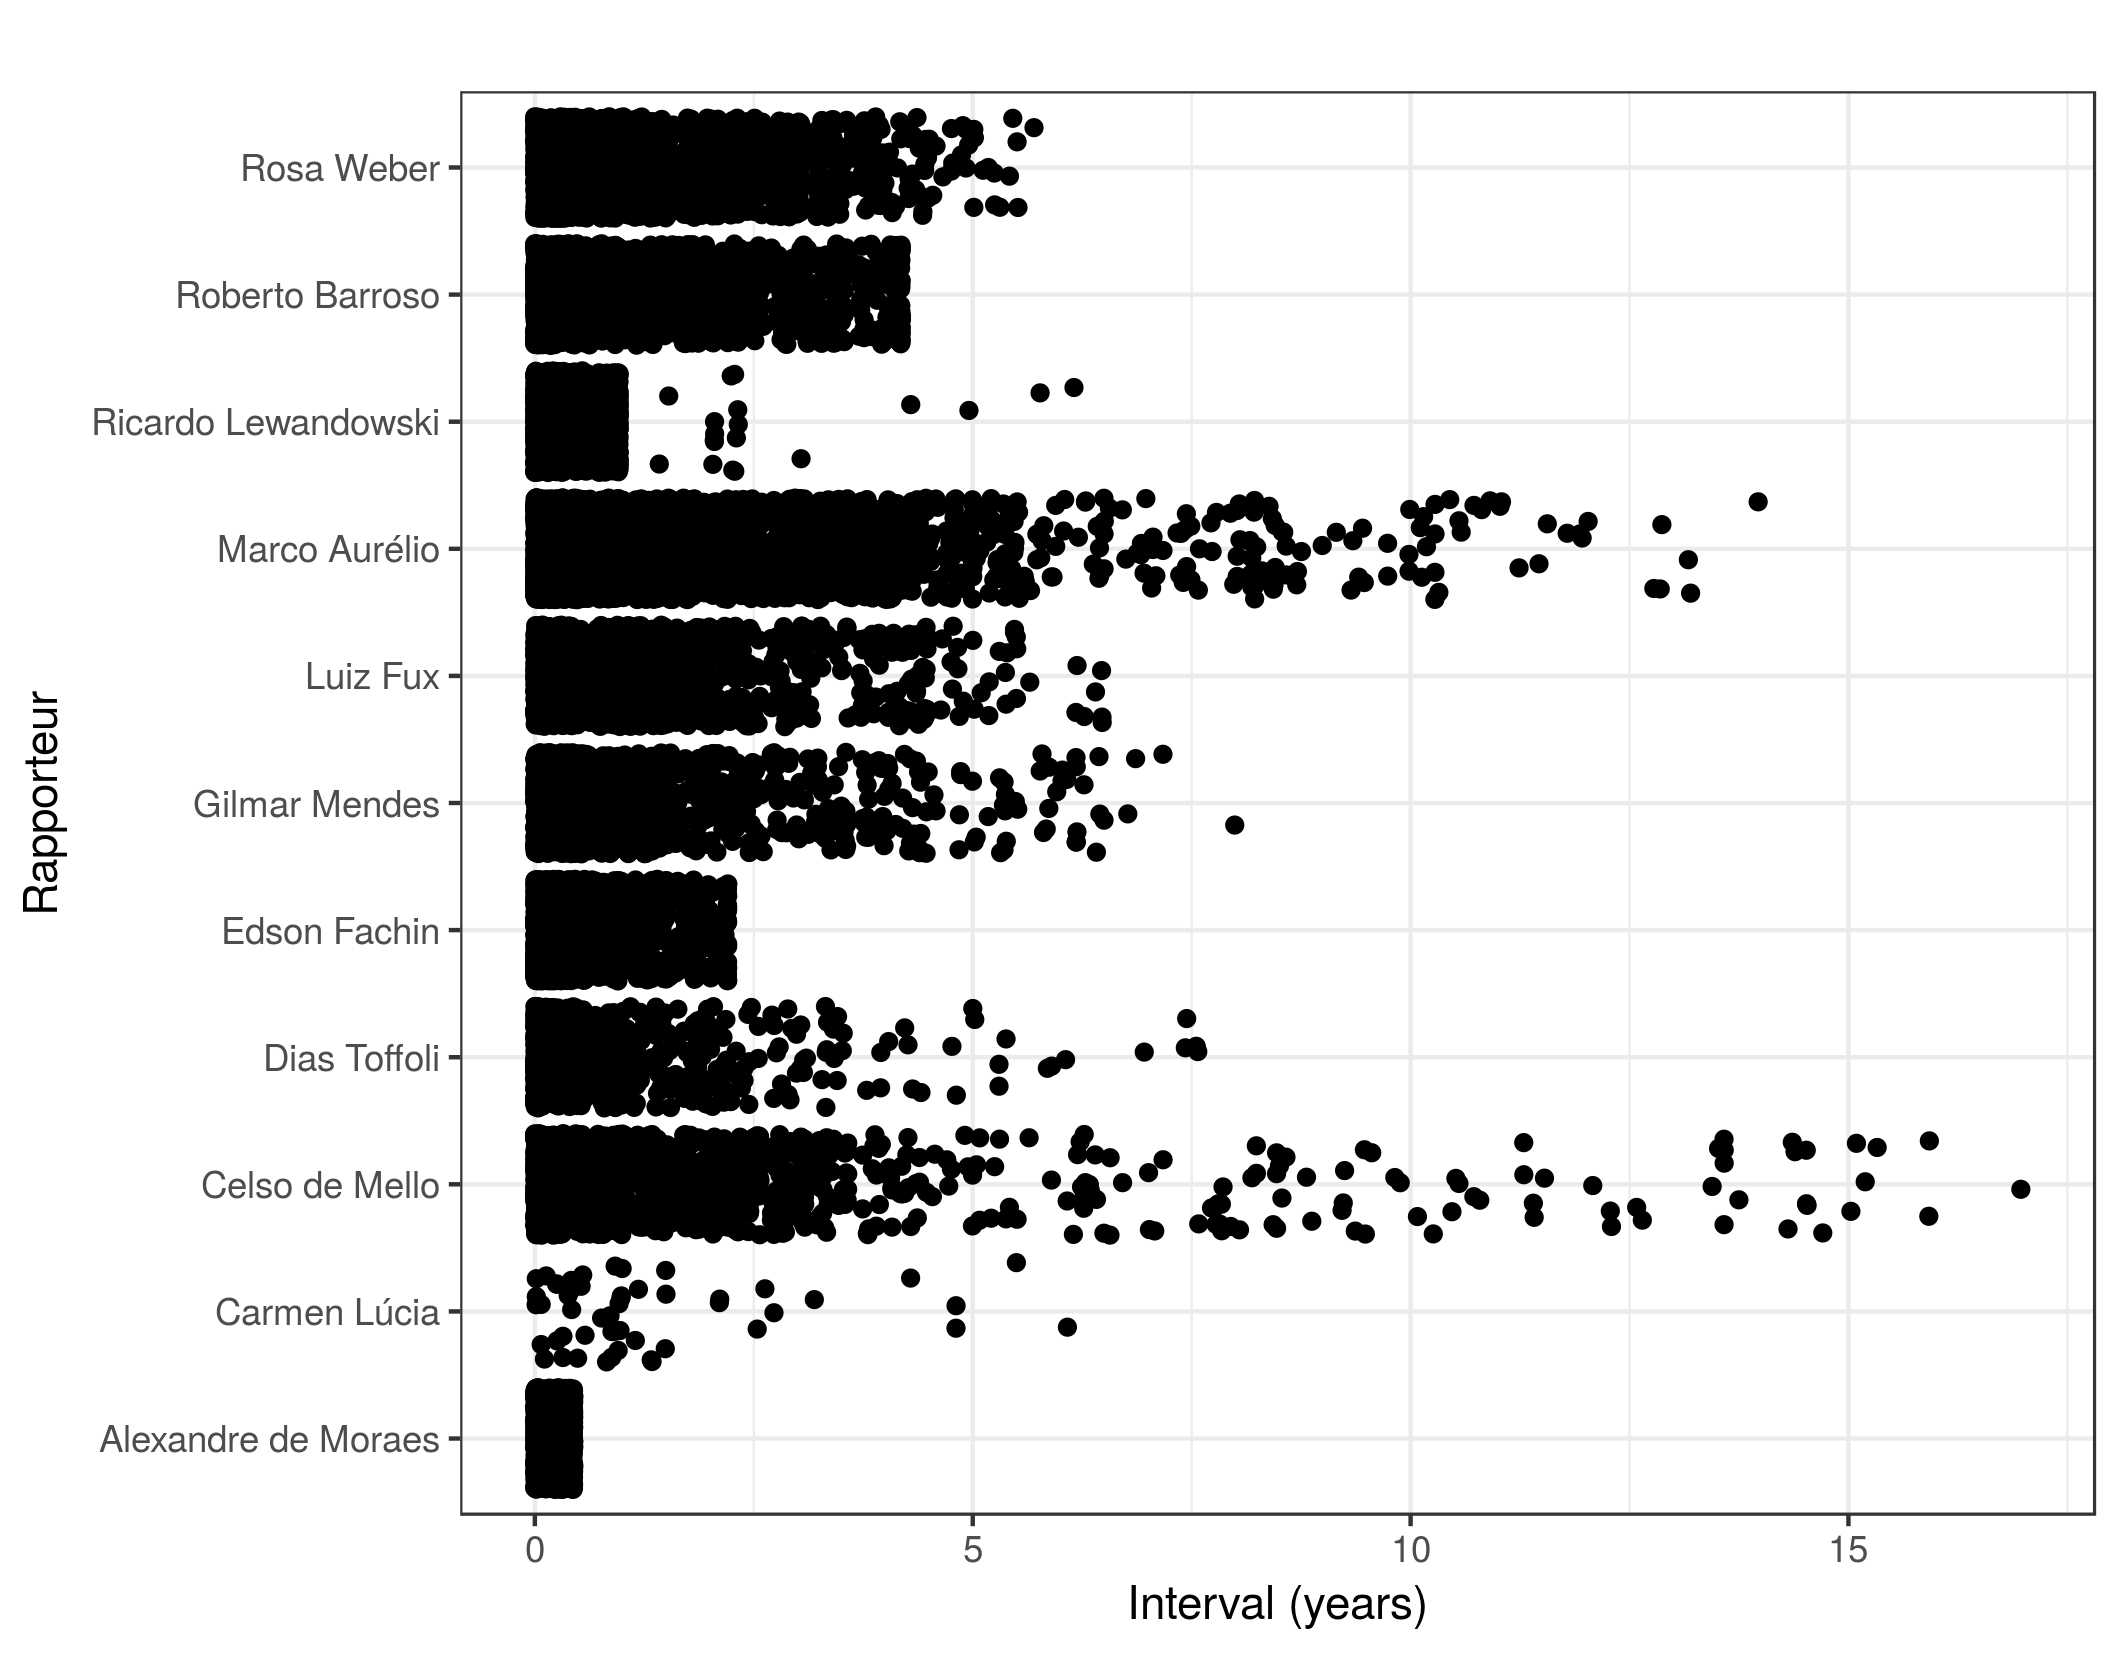
\includegraphics[scale=1]{rapporteur_time.png}
\centering
\end{figure}

Moreover, unlike other players, the rapporteur has the power of changing the \emph{status quo} situation for an action. An important fact about the power of interrupting judgments is that players can only guarantee the \emph{status quo} outcome. The rapporteur, on the contrary, can change this outcome, by making
an individual decision by him/herself. This happens because in some types of lawsuits, including Abstract Judicial Review Controls, justices may make a decision, when the case is urgent. As an illustration, in 2014, justice Luiz Fux took two decisions on a case about allowances to Brazilian judges. This decision reportedly had an impact of 393 millions of dollars, from 2010 to 2014 \citep{auxiliomoradia}. Following his decision, hitherto he  has not submitted the case to be judged by his peers.


\item \emph{The agenda powers of every justice}.

The power to interrupt judgments belongs to every justice. The institutional mechanism which
guarantees this right is called "pedido de vista". When a justice employs this rule, he/she is given time to better study a case before giving her decision. This right is often justified by the great workload of the Court. However, there is no rule that obliges this justice to withdraw
the lawsuit, so  he/she can keep it stopped as long as he/she wishes.  \citet{arguelhes2017timing}  showed that this rule works as an extra-official docket control mechanism. According to the authors, justices employ "pedidos de vista" in order to avoid cases from being judged.
 
Those institutional attributes have not gained much attention from the literature until recent times. Newspapers reportedly assume that the "pedido de vista" is employed by justices strategically when they do not want a lawsuit to be judged. For example, a case about the end of private financing of electoral campaigns was stopped by the justice Gilmar Mendes. Articles in media suggested that he withhold it because he did not agree with the result, since the majority had already been formed \citep{pedidodevistagilmar}.

\end{enumerate}

This suffices to show the extension of agenda-setting in the Brazilian Supreme Court. All in all, individual justices have too much power in comparison to other Courts abroad. They can prevent actions from being judged and, when acting as rapporteurs, make decisions without consulting their peers. In the next section, we formalize how an influencer can use this feature to reach favorable decisions. 




\section{Theory}
\label{theory}

The Brazilian Supreme Court landscape is different from the arguments stated about the American Supreme Court setting. In this section, we review some common results from the literature on majority rule and median voters in Political Science. From our point of view, this theory relies on some assumptions on
how collective behavior is built. In Brazil, however, this result might be contrasted with individual behavior of justices.

\subsection{The Majority Rule and the Median Voter Theorem}

Literature in Political Science has emphasized a common theory, called \emph{median voter theorem}, to explain group choices subjected to the majority rule \citep{black1948rationale}\footnote{See \citet{shepsle1996analyzing} for a didactic explanation}. This theory takes for granted, among others, two important assumptions: a) the first one states that preferences of
actors should follow a common order of preference; b) the second one assumes that preferences of political actors are single-peaked, i. e., there is a point that represents the maximum of their preference. \citet{black1948rationale}
proved, thus, that a majority rule following these assumptions will be the one represented by the median voter. In other words, among the actors, the one whose preference is the median among all the individual preferences, when a majority rule is assumed, will indicate the preference of the group.

To illustrate this point, let us assume that five legislators have to decide a common subject, for instance, the legalization of abortion. We assume that they can have three alternatives or points of preferences: $a_1$) complete legalization, $a_2$) prohibition except in the cases of rape and serious disease, $a_3$) complete prohibition. The first assumption imposes an order of preference, for example, $a_1 < a_2 < a_3$. In this case, $a_1$ is the most preferred alternative for an actor $i$, the assumption implies that he prefers
$a_2$ to $a_3$ as well. The second assumption only states that the actor will have a set of alternative as the most preferable of all. The median voter theorem will consider that for a set of several actors, given a order of preference of the alternatives, if we put them in order, the actor in the middle will mirror any decision in majority rule. If there are three legislators, each one voting for a certain alternative, the one who chose $a_2$ will be the median voter.

Another example is more common in the literature. Assume that preferences might be pinpointed in a Euclidean unidimensional space and five actors have single-peaked utility functions with global maximum distributed over there, as  \autoref{ideologicaldimension} shows. It is quite noticeable that $a_3$ is the median voter in this case.

\begin{figure}[htb]
\label{ideologicaldimension}
\caption{Distribution of single-peaked utility functions across an ideological dimension}
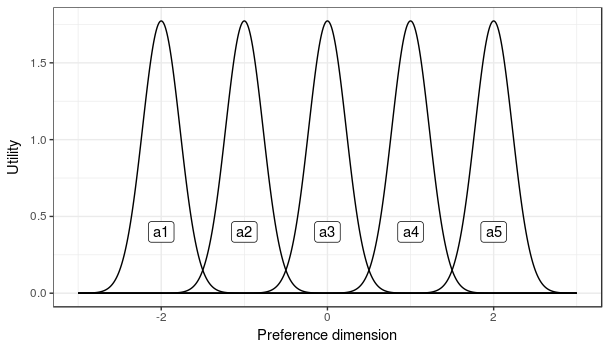
\includegraphics[scale=1]{figure_dimensions.png}
\centering
\end{figure}

As a formalization of the majority rule, this theorem has been quite influential in political science and economics. 

Concerning Judiciary, the median voter theorem has been employed to understand how agents can influence a Court's behavior \citep{martin2004median}. So, if a president  intends to influence the Court, he will probably be pondering how to nominate its median justice or to change it in order to obtain favorable decisions. That is why common strategies concern how to secure a majority in a Court, for example, packing it or removing justices. It is easy to analyze both situations. If there is a Supreme Court with 5 justices and one of them is aligned with the preferences of the government. If the government manages to create more 4 sits in that bench, packing the Court, he can make the initial justice the new median voter. The same logic applies to situations in which justices are impeached. If there are 9 justices and the government manages to influence only 4 of them, by impeaching one of the other five, the government can nominate one more and, hence, it can control the Court.


\subsection{A new model}


For several reasons, we believe that Median Voter Theorem is not suitable to explain the decision-making process in Courts where individual behavior is emphasized. In Brazil, as we have described, lawsuits can commonly be stopped or retarded by justices individually. In addition to this, individual justices might also change the status quo by making decisions. At last, justices do not vote at the same time, but they do so according to a predetermined order. How would an influencer behave in this case? With what strategy would he/she try to influence the Court? For this desideratum, we need a new game theory model. The purpose here is to model the utilities for the influencer and justices of a Court.  

We suppose an influencer, called $i$, representing any actor who would try to influence a result in a Court. We also assume $n$ justices, represented by $j_1, j_2, ..., j_n$. This justice might take a decision $d$. Each of these players have a utility function with a single peak in a Euclidean space.  At last, we consider a specific lawsuit, named $k$.

Each justice utility function is determined by three parameters: \begin{enumerate} \item $\alpha_{jk}(d)$, which represents the stance of a judge regarding a specific decision in a lawsuit. $\alpha_{jk}(d)$ is described by the difference between two points in the Euclidean space, $\alpha_{jk}(d) = x_{jk}(d) - p_{j}$, such that $x$ represents the utility a certain result of a case for the justice, and $p$ the result of greatest utility. $\alpha_{jk}(d)$ is randomly distributed from a normal distribution with mean 0 and variance $\sigma_{\alpha}^2$. \item $\beta_{ji}$, which accounts for the tendency of the judge to agree with a possible influence from $i$. It is obtained from a normal distribution with variance $\sigma_{\beta}^2$ and mean 0. In other words, each justice has a tendency to be subjected to pressure from a certain influencer. \item and $c_{ik}$, accounting for the cost paid by a influencer in a certain case. This parameter is constrained to be positive. The cost might represent any strategy by the influencer to influence a justice, for instance, bribery.  \end{enumerate}  A utility function of a justice is represented by \begin{equation} U_{ijk}(d) = -(x_{jk}(d) - p_{j})^2  + \beta_j c_{ik} \end{equation}.  

We also define the probability of a justice stop a lawsuit by \begin{equation} P(U_{ijk}(d)) = \frac{1}{1+e^{-U_{ijk}(d)}}\end{equation}, such that $d$ means stopping it.


The utility for the influencer is determined by \begin{equation} U_{i} = u_{k}(d)*P_k - c_{i} \end{equation}. $u_{k}(d)$ represent the utility for him/her of a lawsuit $k$ being stopped, $P_k$ the probability of this situation happens, and $c_{i}$, the cost he intends to pay.   He might be a plaintiff or a defendant. Those situations should be understood separately, since they have different implications; however we consider only the second one.

The lawsuit starts and is distributed to a rapporteur $j$, which possess a tendency $\beta_{ji}$. $i$ is an actor with strong interest in a certain result for this lawsuit. He/she believes that the Court might take a decision against him and intends to stop or retard this case. In other words, he will only do that if he considers that the probability of stopping a case times the utility of it is higher than the a possible cost. If not, the solution is trivial, and he will not try to influence the Court. Since cost might be high for a possible influence, this situation seems to be the most common in the Brazilian Supreme Court.  

However , if the influencer intends to influence a justice, he/she will consider its beliefs about the probability of obtaining a favorable decision. \autoref{modelo-grafico} shows the probability, given certain values for the parameters.


\begin{figure}[htb]
\label{modelo-grafico}
\caption{Probability of a justice stopping a lawsuit }
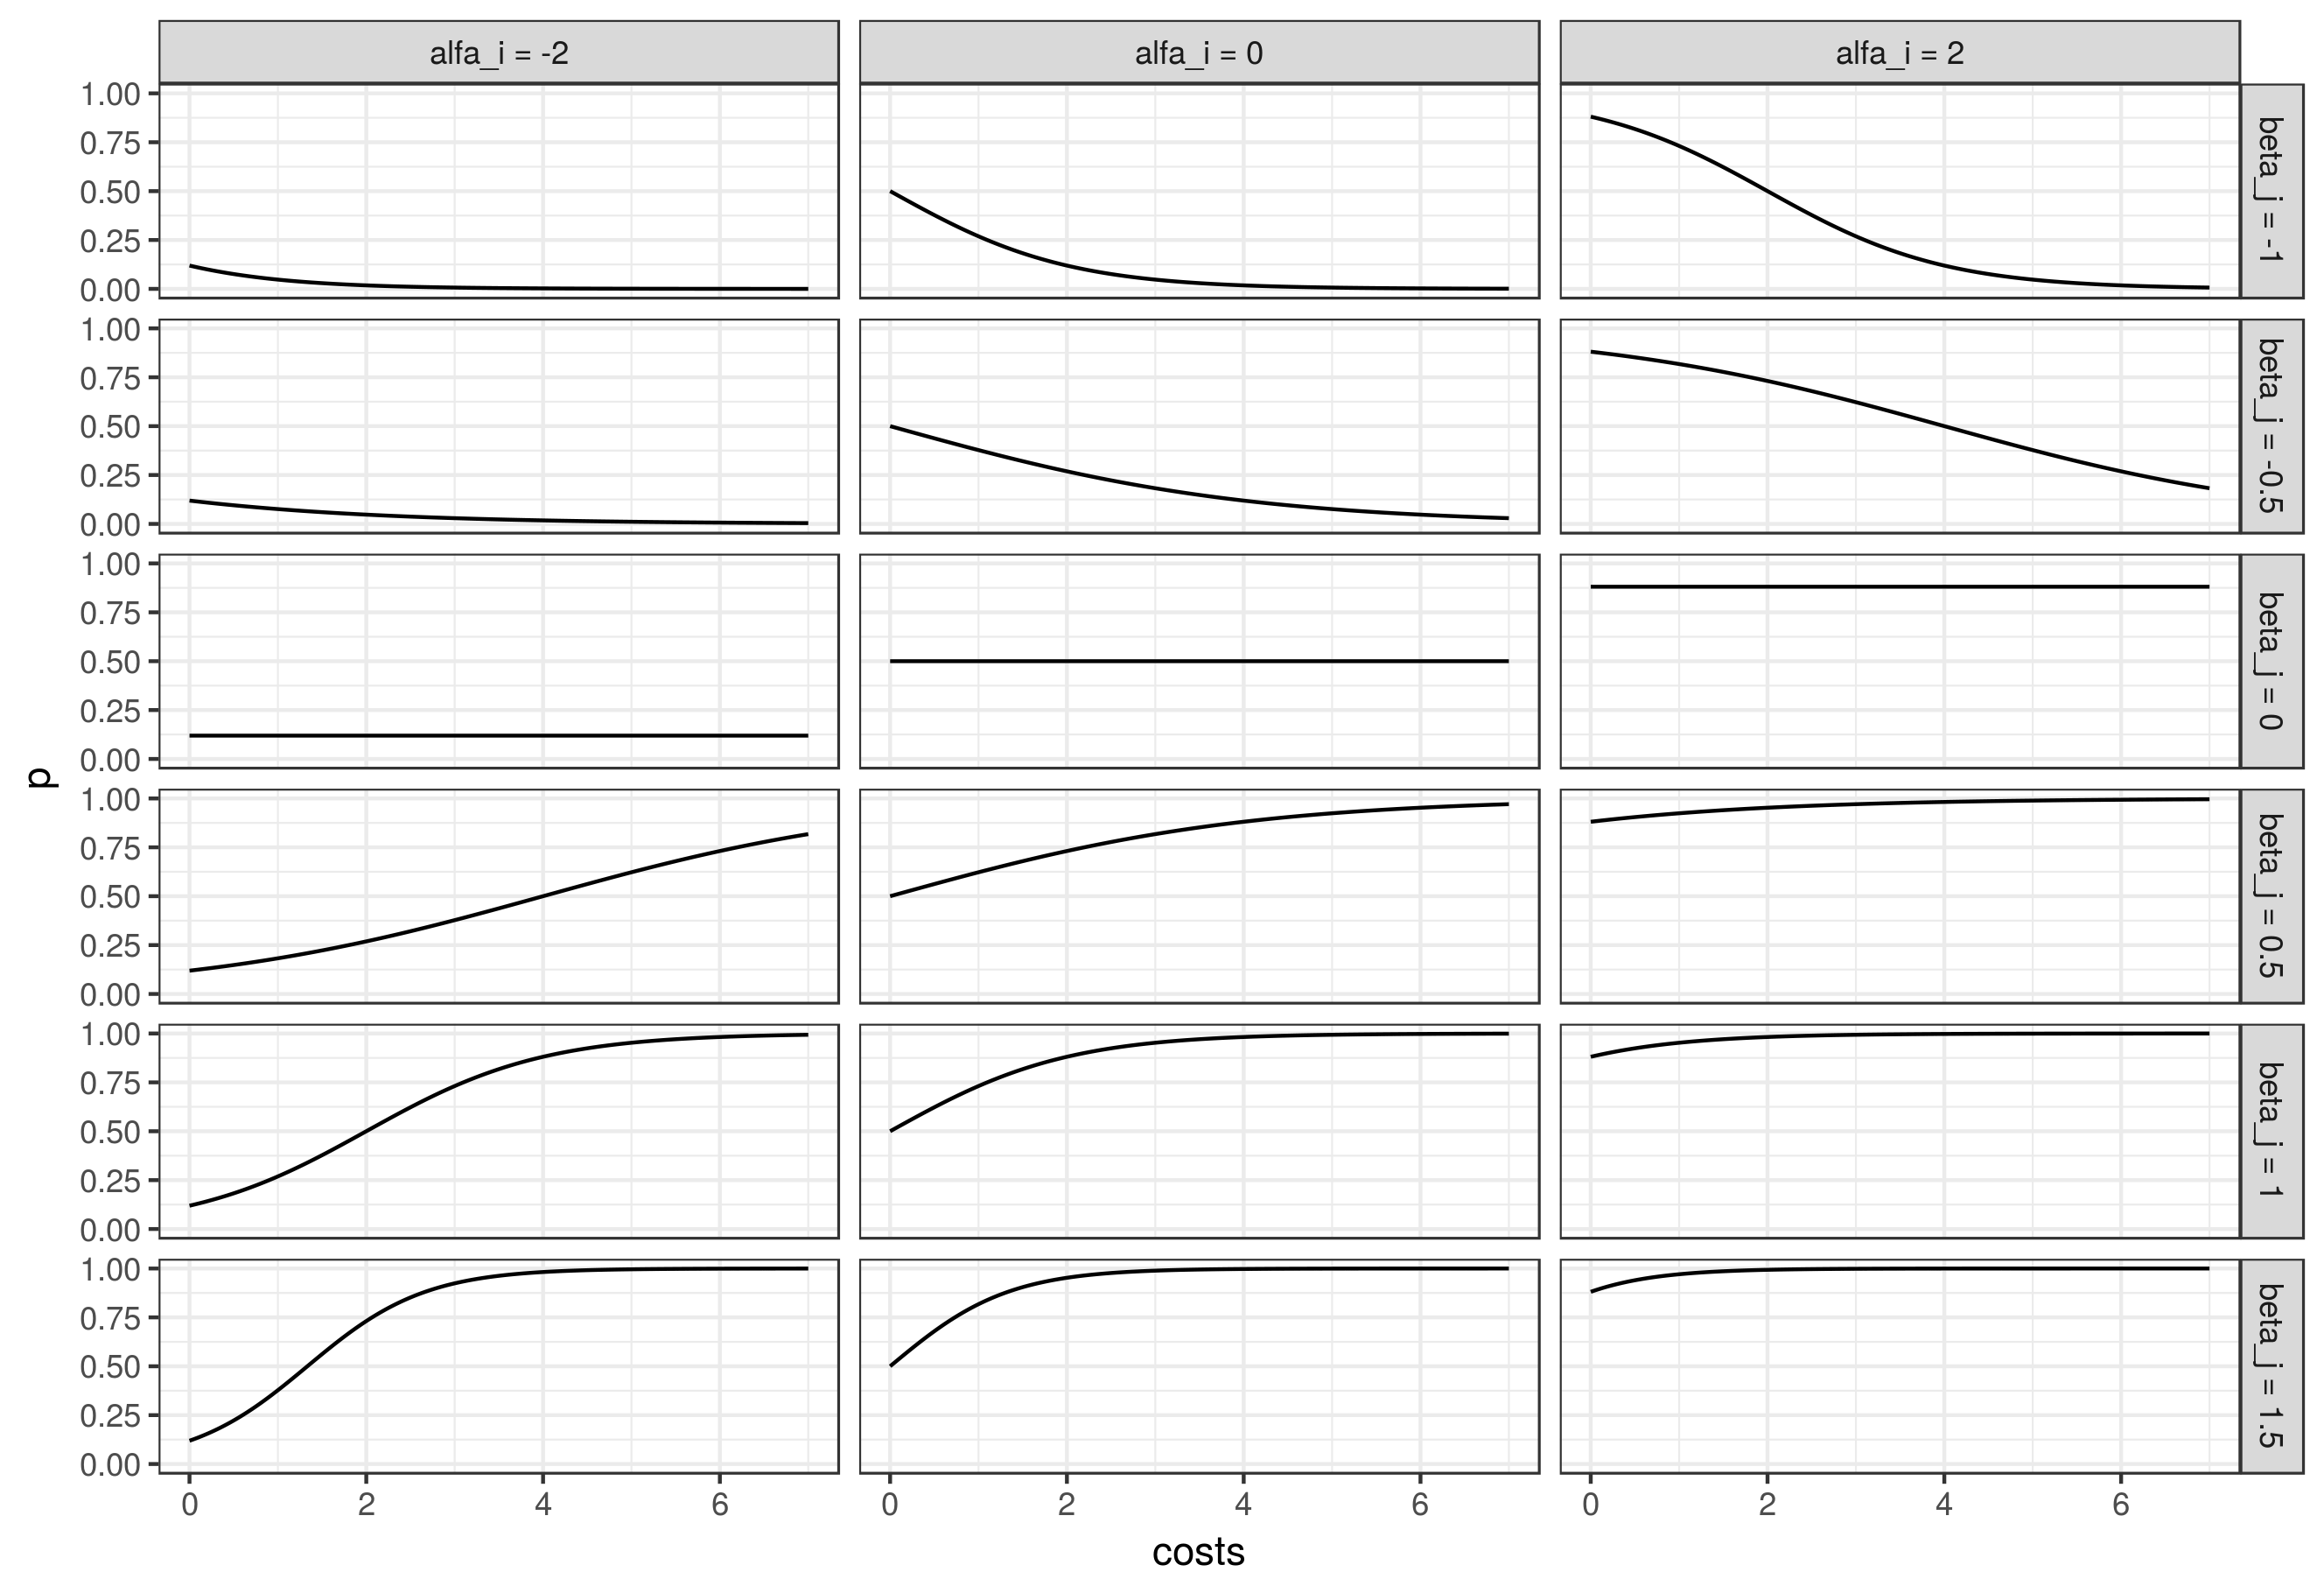
\includegraphics[scale=.8]{modelo.png}
\centering
\end{figure}

This model implies a few hypothesis (proofs in the appendix): \begin{hypothesis} \item \emph{The influencer will only try to influence those justices who, he thinks, have a positive tendency to being influenced.} \item \emph{If the influencer can only choose one justice to influence, he/she will try to influence that one with the greatest value for $\beta$, given the constraint of H1, if justices have the same tendency to stop a lawsuit. } \item \emph{Regardless of the value of $\alpha$, the influencer will try to influence the justice whose $\beta$ is higher.} \item \emph{Depending on the cost, it is reasonable to assume that two or three justices are sufficient to guarantee that a probability of a case being stopped is close to 1 }  \end{hypothesis}

All in all, our model shows that, in environment where majority rule is present, but individual behavior is emphasized, influencing one or two justices are sufficient to control the whole Court. This fact has an strong implication for judicial independence studies, since it is needless to employ strategies as packing the Court or removing judges to have a strong influence.

In Brazil, at least after the Constitution of 1988, there are no cases in which justices were removed and it is quite noticeable that the president does not care for a strong identification. This evidence is in complete accordance to what our model would predict. 

%\section{Case Studies}

%In this section, we will discuss some cases in Brazil that fit our model. It is not easy to test it, using %quantitative data. The main problem is there is not sufficient data to build a robust statistical model. %Qualitatively, it is also difficult to test it, because there does not exist reliable manner of %identifying lobby is happening. We rely exclusively on what newspaper presumes.

%\subsection{Allowances for judges in Brazil}

%Salaries for legal public careers are not clearly established. They have to follow a clear limit, which is the salary for a justice of the Supreme Court. However, in order to eschew those limits, judges and judicial associations started to employ types of allowances to pay costs of house renting, food and other benefits.
 
%It has been a discussion if those allowances are constitutional. 

\section{Discussion}

In face to the model employed, there are a couple of consequences for Brazilian Supreme Court. Firstly, we have to consider that it is easy to influence a justice and, consequently, the whole Court in Brazil. Then, if the drawn model is correct, we should take into account that the external judicial independence of the Court is low, in opposition to those who argue otherwise. It is quite easy for an agent, including the president, to stop an unfavorable lawsuit against him/her.

Additionally, some cases exemplify our model. In 2014, an lawsuit defied the system of campaign financing in Brazil. Plaintiffs argued that Brazilian Constitution would forbid financing by companies and firms. After 6 justices voted, a majority had been constituted in favor of the prohibition. Knowing that the result was inevitable, one of the justices, Gilmar Mendes, decided to stop the lawsuit. Then, the \textit{status quo} was kept, even though the majority of the justices had reached a conclusion. Although some journalists claimed there was an intervention by some public agents, this will never be clear. However, considering that one justice was able to stop the lawsuit, we suggest that this fact validates our model.

This is not the only case. For example, In 2017, a case questioned the "foro privilegiado", a perquisite that public agents have in Brazil to be judged only by high Courts. It is widely considered that this perquisite is advantageous to politicians, since high Courts are not well suitable to handle criminal cases. This case had the support of the majority of the Court. Justice Dias Toffoli decided, then, to stop the lawsuit. Again, \textit{status quo} was maintained. 

Although it is not clear if agents always try to influence Court, this hypothesis is plausible. Hence, we might conclude that judicial independence of the Brazilian Court is low. 




\bibliography{biblio}

\end{document}